\section{Resultados}

\hspace{0.4cm}Nesta seção serão apresentados os resultados obtidos para as diferentes bases de dados, além de suas implicações.

\subsection{Ferramenta computacional ProLoss}

\hspace{0.4cm}Tratando da estrutura do código da ferramenta computacional, como dito anteriormente, as funções de cálculo foram moduladas e divididas, de forma que os itens auxiliares, as perdas imediatas e as perdas progressivas possuem seu próprio diretório, como podem ser vistas na Figura \ref{fig:arvore_de_arquivos}.

\begin{figure}[h!]
    \centering
    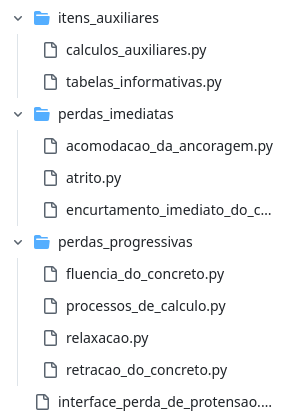
\includegraphics[width=0.45\textwidth]{imgs/arvore_de_arquivos.png}
    \caption{Árvore de arquivos do código fonte.}
    \label{fig:arvore_de_arquivos}
    \medskip
    \small Fonte: Elaboração Própria (2024).
\end{figure}\bigskip

Como mencionado, elas foram pensadas e programadas de forma que ficassem de fácil acesso para auditoria do código do cálculo, e independentes da interface gráfica. Esta, ficou em um arquivo separado no mesmo nível dos diretórios de cálculo, onde importa todas as funções e integra os dados inseridos pelos usuários, os cálculos realizados nas funções e o resultado exposto na tela. O código com essas importações, além das outras bibliotecas utilizadas para operação da ferramenta podem ser vistos na Listagem \ref{lst:imports}.
\bigskip


\begin{lstlisting}[caption={Importações de funções de cálculo e outras bibliotecas no código fonte}, label={lst:imports}]
import tkinter as tk

import os
import sys
import base64

from tkinter import *
from tkinter import ttk
from tkinter.filedialog import askopenfilename
from matplotlib.backends.backend_tkagg import FigureCanvasTkAgg

import matplotlib.pyplot as plt
import pandas as pd
import numpy as np

from perdas_imediatas.atrito import atrito
from perdas_imediatas.acomodacao_da_ancoragem import acomodacao_da_ancoragem
from perdas_imediatas.encurtamento_imediato_do_concreto import encurtamento_imediato_do_concreto

from itens_auxiliares.tabelas_informativas import tabelas_informativas
from itens_auxiliares.calculos_auxiliares import calculo_da_espessura_ficticia
from itens_auxiliares.calculos_auxiliares import calculo_da_idade_ficticia
from itens_auxiliares.calculos_auxiliares import efeito_conjunto_retracao_e_fluencia

from perdas_progressivas.retracao_do_concreto import retracao_do_concreto
from perdas_progressivas.fluencia_do_concreto import fluencia_do_concreto
from perdas_progressivas.fluencia_do_concreto import superposicao_de_efeitos
from perdas_progressivas.relaxacao import relaxacao_pura
from perdas_progressivas.relaxacao import relaxacao_relativa
from perdas_progressivas.processos_de_calculo import perda_progressiva_processo_simplificado
from perdas_progressivas.processos_de_calculo import perda_progressiva_metodo_geral
\end{lstlisting}
\vspace{-2.1em}
\medskip
\begin{center}
\small Fonte: Elaboração Própria (2024).
\end{center}

Em relação as telas, as principais foram divididas em abas e definidas como os cálculos principais das perdas de protensão imediatas e progressivas. A primeira aba trata-se da perda de protensão imediata por atrito através de processo simplificado, descrita pela sigla de PIAT, como pode ser visto na Figura \ref{fig:piat}.\bigskip

\begin{figure}[h!]
    \centering
    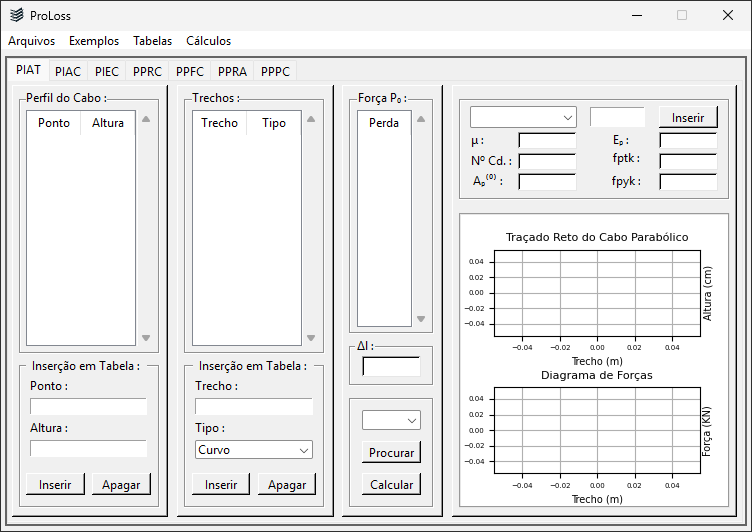
\includegraphics[width=0.85\textwidth]{imgs/piat.png}
    \caption{Perda de protensão imediata por atrito através de processo simplificado.}
    \label{fig:piat}
    \medskip
    \small Fonte: Elaboração Própria (2024).
\end{figure}

A segunda aba se refere a perda de protensão imediata por acomodação de ancoragem, representada pela sigla PIAC e presente na Figura \ref{fig:piac}

\newpage

\begin{figure}[h!]
    \centering
    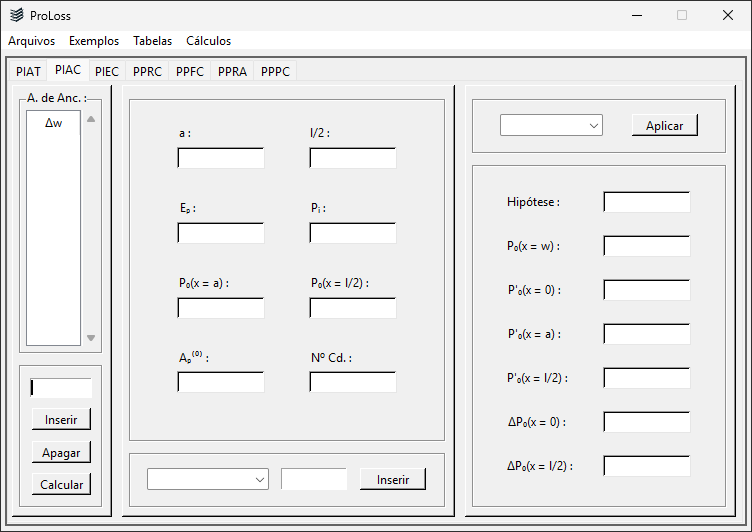
\includegraphics[width=0.85\textwidth]{imgs/piac.png}
    \caption{Perda de protensão imediata por acomodação de ancoragem.}
    \label{fig:piac}
    \medskip
    \small Fonte: Elaboração Própria (2024).
\end{figure}

A terceira aba se refere ao último tipo de cálculo de perda imediata da ferramenta, que é a perda de protensão por encurtamento imediato do concreto, a PIEC, e pode ser visualizada na Figura \ref{fig:piec}.\bigskip

\begin{figure}[h!]
    \centering
    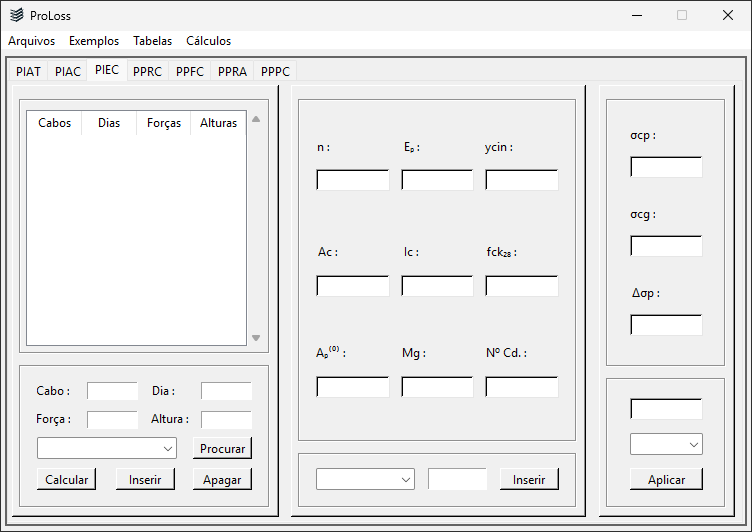
\includegraphics[width=0.85\textwidth]{imgs/piec.png}
    \caption{Perda de protensão por encurtamento imediato do concreto.}
    \label{fig:piec}
    \medskip
    \small Fonte: Elaboração Própria (2024).
\end{figure}

A soma do resultado das três abas, a depender do cálculo que o projetista irá realizar, pode representar justamente a perda imediata de protensão total da estrutura. Seguindo para as perdas progressivas, têm-se a quarta aba que se refere ao cálculo da retração do concreto, que compõe a fluência no cálculo do efeito conjunto no concreto. Ela é descrita pela sigla PPRC, como observada na Figura \ref{fig:pprc}.\bigskip

\newpage

\begin{figure}[h!]
    \centering
    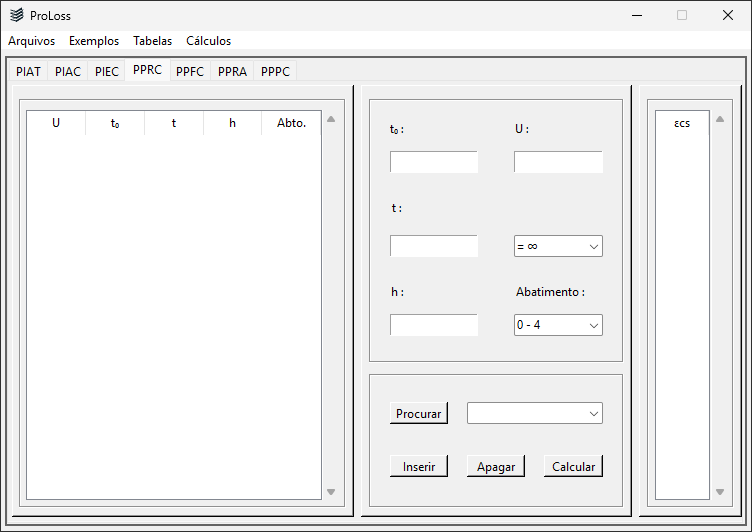
\includegraphics[width=0.85\textwidth]{imgs/pprc.png}
    \caption{Cálculo da retração do concreto.}
    \label{fig:pprc}
    \medskip
    \small Fonte: Elaboração Própria (2024).
\end{figure}

A quinta aba trata do cálculo da fluência do concreto, e como dito anteriormente, fará parte do cálculo do efeito conjunto em uma tela para cálculos auxiliares que será vista posteriormente. A aba é representada pela sigla PPFC e pode ser vista na Figura \ref{fig:ppfc}.\bigskip

\begin{figure}[h!]
    \centering
    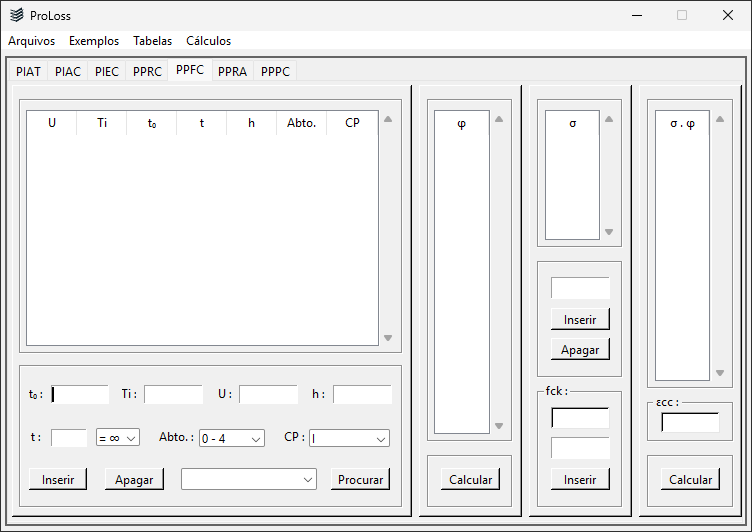
\includegraphics[width=0.85\textwidth]{imgs/ppfc.png}
    \caption{Cálculo da fluência do concreto.}
    \label{fig:ppfc}
    \medskip
    \small Fonte: Elaboração Própria (2024).
\end{figure}

A sexta aba promove o cálculo da relaxação pura e relativa. Destaca-se que a relaxação relativa quando utilizada com o efeito conjunto da retração e fluência, possibilita o cálculo da perda de protensão progressiva pelo método geral. A sigla da aba é a PPRA, visualizada na Figura \ref{fig:ppra}.\bigskip

\newpage

\begin{figure}[h!]
    \centering
    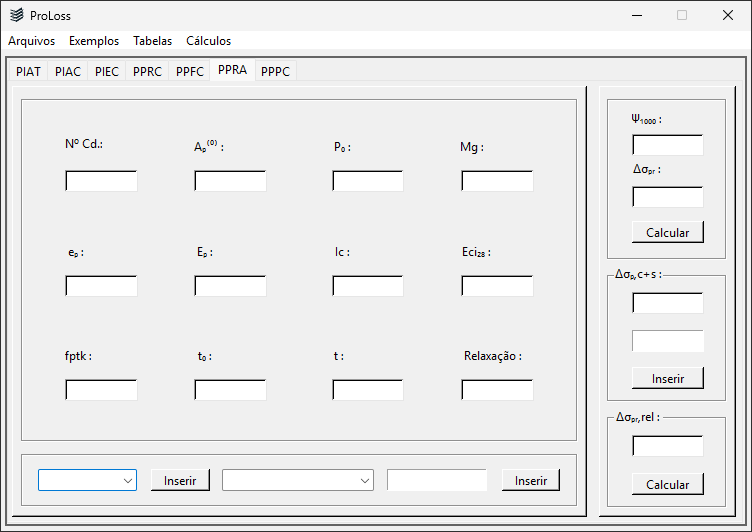
\includegraphics[width=0.85\textwidth]{imgs/ppra.png}
    \caption{Cálculo da relaxação pura e relativa.}
    \label{fig:ppra}
    \medskip
    \small Fonte: Elaboração Própria (2024).
\end{figure}

Ressalta-se que para a realização dos cálculos das abas das Figuras \ref{fig:pprc}, \ref{fig:ppfc} e \ref{fig:ppra} serão necessários cálculos auxiliares que terão suas telas vistas posteriormente, da idade e espessura fictícia. A sétima e última aba permitirá o cálculo da perda de protensão progressiva pelo método geral, ou pelo processo simplificado. Sua sigla é PPPC, e ela pode ser observada na Figura \ref{fig:pppc}.\bigskip

\begin{figure}[h!]
    \centering
    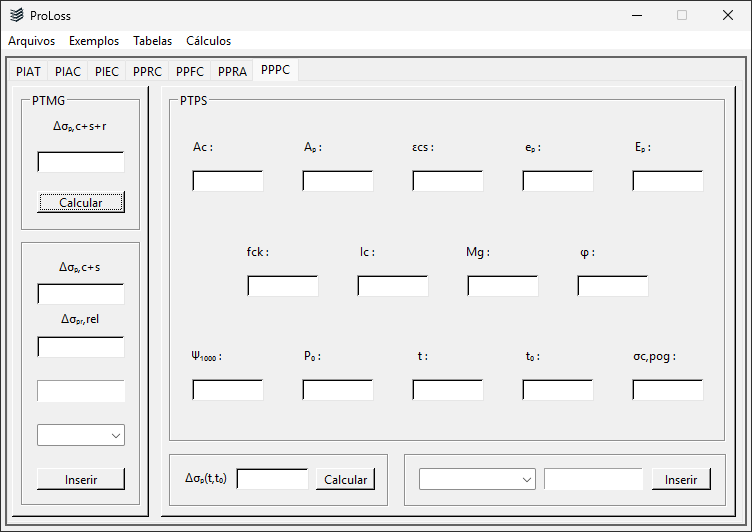
\includegraphics[width=0.85\textwidth]{imgs/pppc.png}
    \caption{Cálculo da perda de protensão progressiva pelo método geral e processo simplificado.}
    \label{fig:pppc}
    \medskip
    \small Fonte: Elaboração Própria (2024).
\end{figure}

Faz-se necessário salientar que, caso o usuário opte pelo cálculo das perdas de protensão progressiva pelo método simplificado, apenas a aba da Figura \ref{fig:pppc} será necessária, através das variáveis presentes na parte da janela representada pela sigla PTPS. Já se o método geral for o preterido, necessitar-se-á dos cálculos das abas das Figuras \ref{fig:pprc} e \ref{fig:ppfc} aliados ao efeito conjunto de retração e fluência, além dos cálculos da aba da Figura \ref{fig:ppra}. A parte da janela que trata do método geral é composta pela sigla PTMG, na tela da da Figura \ref{fig:pppc}. 

Partindo para os itens da barra de ferramentas acima das abas, o primeiro deles é chamado Arquivos. Através de seus objetos é possível limpar todas as variáveis preenchidas, reiniciar a ferramenta computacional, abrir uma tela com informações sobre a ferramenta computacional, ou sair da mesma. Eles podem ser vistos na Figura \ref{fig:arquivos}.\bigskip

\begin{figure}[h!]
    \centering
    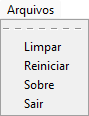
\includegraphics[width=0.15\textwidth]{imgs/arquivos.png}
    \caption{Arquivos, da barra de ferramentas.}
    \label{fig:arquivos}
    \medskip
    \small Fonte: Elaboração Própria (2024).
\end{figure}

O segundo item da barra de ferramentas é chamado de exemplos, e nele contém exemplos retirados do livro de Cholfe e Bonilha (\citeyear{CB}) e resolvidos. Existem exemplos para cada um dos cálculos auxiliares, de perdas imediatas e progressivas, conferidos com os resultados do livro. É possível distinguir cada um deles a partir da sigla qual ele se refere, e no código fonte onde estão dispostos os exemplos também há a referência da página exata de onde ele foi retirado do livro, para fins de aferição. É possível observar o item chamado exemplos a partir da Figura \ref{fig:exemplos}.\bigskip

\begin{figure}[h!]
    \centering
    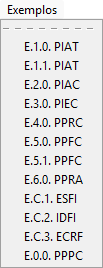
\includegraphics[width=0.15\textwidth]{imgs/exemplos.png}
    \caption{Exemplos, da barra de ferramentas.}
    \label{fig:exemplos}
    \medskip
    \small Fonte: Elaboração Própria (2024).
\end{figure}

Seguindo para a terceira aba tem-se o item de tabelas. O primeiro objeto dele é chamado de siglas, e contém uma tela com o significado de todas as siglas usadas na ferramenta computacional. Logo após, vêm o objeto chamado variáveis, que segue a mesma lógica das siglas, porém informa todas as variáveis, seus significados e as unidades de medida de cada uma delas. Segue-se então para os últimos dois objetos chamados fluência e retração, e endurecimento do cimento. Eles dispõem de duas telas com gráficos que podem vir a auxiliar os projetistas nos cálculos da ferramenta computacional, de forma a promover uma maior facilidade de consultar, não precisando sair da ferramenta e recorrer à algum outro documento. Visualiza-se o item tabelas na Figura \ref{fig:tabelas}.\bigskip

\newpage

\begin{figure}[h!]
    \centering
    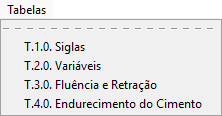
\includegraphics[width=0.35\textwidth]{imgs/tabelas.png}
    \caption{Tabelas, da barra de ferramentas.}
    \label{fig:tabelas}
    \medskip
    \small Fonte: Elaboração Própria (2024).
\end{figure}

Por fim na barra de ferramentas têm-se o item de cálculos, que dispõe de objetos que resultaram em telas para permitir os cálculos complementares, como observado na Figura \ref{fig:calculos}.\bigskip

\begin{figure}[h!]
    \centering
    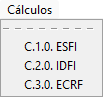
\includegraphics[width=0.15\textwidth]{imgs/calculos.png}
    \caption{Cálculos, da barra de ferramentas.}
    \label{fig:calculos}
    \medskip
    \small Fonte: Elaboração Própria (2024).
\end{figure}

O primeiro objeto do item cálculos da barra de ferramentas trata-se do cálculo auxiliar da espessura fictícia, descrita pela sigla ESFI e com sua tela vista na Figura \ref{fig:espessura_ficticia}.\bigskip

\begin{figure}[h!]
    \centering
    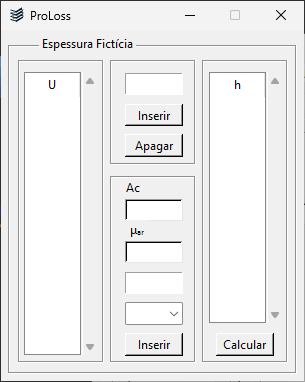
\includegraphics[width=0.45\textwidth]{imgs/espessura_ficticia.png}
    \caption{Cálculo da espessura fictícia.}
    \label{fig:espessura_ficticia}
    \medskip
    \small Fonte: Elaboração Própria (2024).
\end{figure}

Já o segundo objeto do item cálculos é o cálculo auxiliar da idade fictícia, de sigla IDFI. Junto da espessura fictícia representada na Figura \ref{fig:espessura_ficticia}, eles podem ser usados para auxiliar cálculos como a da relaxação pura e relativa. Visualiza-se a tela da idade fictícia a partir da Figura \ref{fig:idade_ficticia}.\bigskip

\newpage

\begin{figure}[h!]
    \centering
    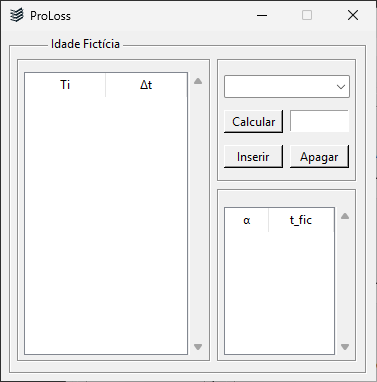
\includegraphics[width=0.52\textwidth]{imgs/idade_ficticia.png}
    \caption{Cálculo da idade fictícia.}
    \label{fig:idade_ficticia}
    \medskip
    \small Fonte: Elaboração Própria (2024).
\end{figure}

O terceiro e último objeto do item cálculos é o cálculo auxiliar do efeito conjunto da retração e fluência. Ele é importante em especial para os usuários que optarem por cálcular as perdas progressivas pelo método geral, como explicado anteriormente. A sigla que define o objeto é ECRF, e sua tela pode ser observada a partir da Figura \ref{fig:ecrf}.\bigskip

\begin{figure}[h!]
    \centering
    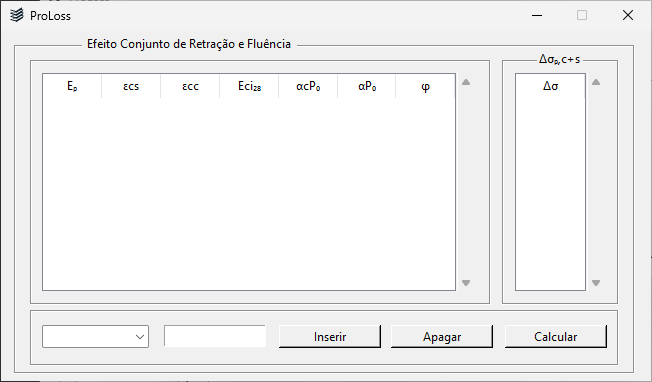
\includegraphics[width=0.85\textwidth]{imgs/ecrf.png}
    \caption{Cálculo do efeito conjunto da retração e fluência.}
    \label{fig:ecrf}
    \medskip
    \small Fonte: Elaboração Própria (2024).
\end{figure}

\subsection{Validação da ferramenta computacional}

\hspace{0.4cm}A validação da ferramenta ocorreu por meio da comparação do resultado dos exemplos do livro resolvidos através da ferramenta computacional, onde todos os métodos e funções de cálculo implementados na ferramenta foram testados. Assim, é avaliado para os resultados calculados no livro e na ferramenta as diferenças absolutas e relativas entre os dois, de forma a entender se as diferenças nos resultados são apenas diferenças de aproximação, e se são relevantes para considerar ou não o uso da ferramenta. 

\subsubsection{Exemplo de aplicação numérica para cálculo de perdas imediatas de protensão por atrito através de processo simplificado}

\hspace{0.4cm}A aplicação numérica para o cálculo das perdas imediatas, trata-se de uma questão que se propõe a calcular a partir dos cabos de uma laje maciça, as perdas por atrito e o alongamento teórico (Cholfe e Bonilha, \citeyear{CB}, p. 142). Os cabos se alongam por seis seções divididas a partir de sete pontos que vão de A à G. Após os cálculos, é possível ver os resultados no gráfico do diagrama de forças da Figura \ref{fig:diagrama_de_forças}.\bigskip

\begin{figure}[h!]
    \centering
    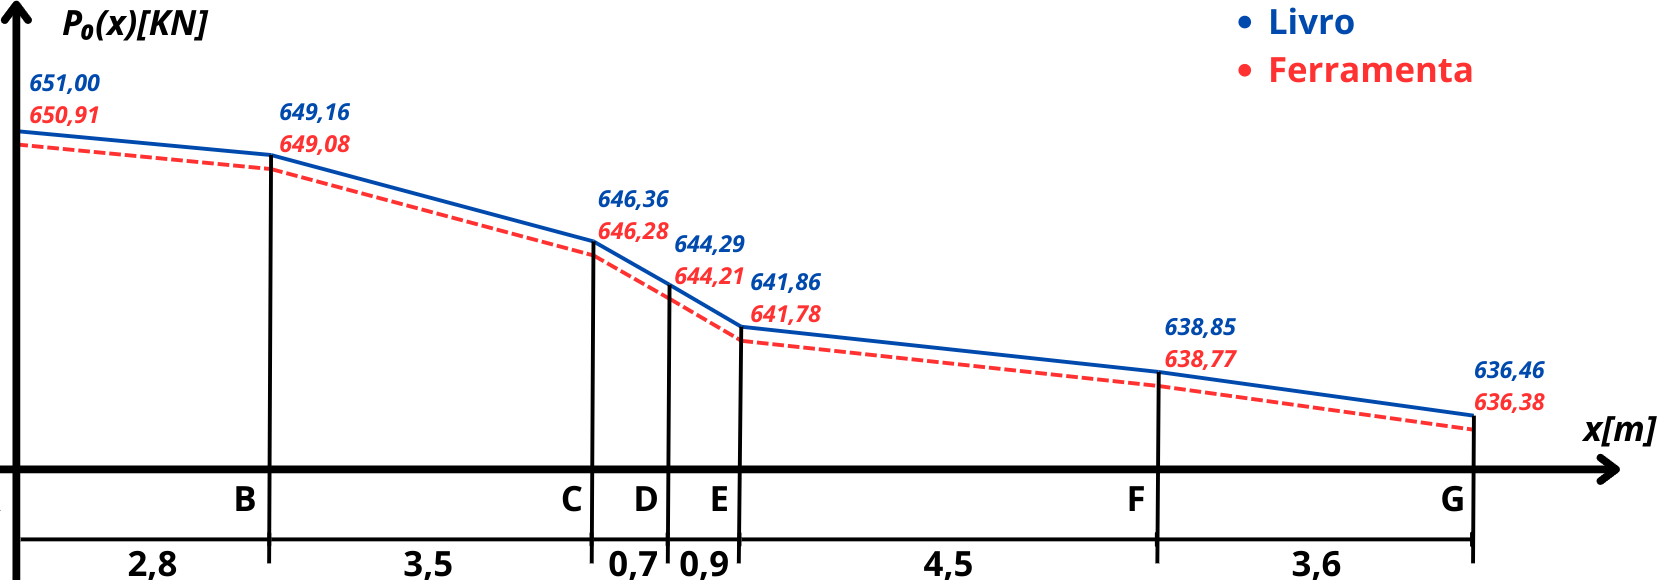
\includegraphics[width=0.9\textwidth]{imgs/diagrama_de_forças.png}
    \caption{Diagrama de forças considerando os resultados do livro e da ferramenta.}
    \label{fig:diagrama_de_forças}
    \medskip
    \small Fonte: Elaboração Própria (2024).
\end{figure}

Através do gráfico da Figura \ref{fig:diagrama_de_forças} observa-se os valores das perdas dos trechos. As diferenças absolutas e relativas de todos os trechos são iguais considerando, sendo de 0,8 e 0,1\% respectivamente, para duas casas de precisão, além de serem muito baixos, visto que a diferença relativa se mantém como 0,01\%. Em relação ao alongamento teórico obtido das perdas, o valor do exemplo foi de 122,56mm enquanto o da ferramente foi de 122,79mm, com uma diferença absoluta de 0,23mm, com uma diferença relativa de aproximadamente 0,19\%, relevando também resultados muito próximos.

\subsubsection{Exemplo de aplicação numérica para cálculo de perdas imediatas de protensão por acomodação de ancoragem}

\hspace{0.4cm}Para acomodação de ancoragem, a aplicação numérica apresenta um exemplo de um cabo com seis cordoalhas, com ancoragens ativas e passivas. A partir dos dados do exemplo, espera-se determinar as perdas por atrito e a acomodação da ancoragem ativa (Cholfe e Bonilha, \citeyear{CB}, p. 151). Dados os requisitos da questão, foram realizados cálculos para acomodações de ancoragem de 2 e 3,5 milímetros.

Para uma acomodação de 2 milímetros, a hipótese 1 foi satisfeita, e os resultados obtidos tanto pelo livro quanto pela ferramenta numérica foram idênticos, apresentando valores de $Po(x=w)$ iguais a 1105,91 kN, $P'o(x=0)$ iguais a 1034,14 kN e $\Delta P(x = 0)$ iguais a 143,54 kN. Não houve diferença significativa entre os valores calculados, com diferenças absolutas e relativas iguais a zero, indicando uma correspondência exata entre os métodos. Seguindo para a acomodação de 3,5 milímetros, a hipótese 2 foi satisfeita, e os resultados podem ser vistos na Tabela \ref{tab:perdas_piac_3}.

\begin{table}[h!]
\centering
\begin{tabular}{ccccc}
\hline
Variáveis & Livro & Ferramenta & Diferença Absoluta & Diferença Relativa \\ \hline
Po(x = w) & 1085,00 kN & 1084,99 kN & 0,01  kN & 0,00\% \\
P’o(x = 0) & 992,32 kN & 992,31 kN & 0,01 kN & 0,00\% \\
P’o(x = a) & 1076,62 kN & 1076,62 kN & 0,00 kN & 0,00\% \\
$\Delta$Po(x = 0) & 185,36 kN & 185,37 kN & 0,01 kN & 0,00\% \\ \hline
\end{tabular}
\caption{\label{tab:perdas_piac_3} Resultados para cálculos de perdas por acomodação de acoragem de 3mm.}Fonte: Elaboração Própria (2024).
\end{table}

Os resultados da Tabela \ref{tab:perdas_piac_3} foram semelhantes aos encontrados no exemplo para acomodação de 2 milímetros, no aspecto de que a diferença absoluta foi ínfima, gerando diferenças relativas iguais de zero por cento para duas casas decimais.

\subsubsection{Exemplo de aplicação numérica para cálculo de perdas de protensão por encurtamento imediato do concreto}

\hspace{0.4cm}A aplicação numérica para as perdas por encurtamento imediato do concreto usa um exemplo de estrutura com uma viga protendida com dez cabos em pós-tração (Cholfe e Bonilha, \citeyear{CB}, p. 155). Os resultados do cálculo das perdas médias tanto no livro como na ferramenta são apresentados na Tabela \ref{tab:perdas_piec}.

\begin{table}[h!]
\centering
\begin{tabular}{ccccc}
\hline
Variáveis & Livro & Ferramenta & Diferença Absoluta & Diferença Relativa \\ \hline
$\sigma$cp & -11549,59 kPa & -11549,59 kPa & 0,00 kPa & 0,00\% \\
$\sigma$cg & 3315,00 kPa & 3315,00 kPa & 0,00 kPa & 0,00\% \\
$\Delta\sigma$p & -22147,75 kPa & -22148,02 kPa & 0,27 kPa & 0,00\% \\ \hline
\end{tabular}
\caption{\label{tab:perdas_piec} Resultados para cálculos de perdas por encurtamento imediato do concreto.}Fonte: Elaboração Própria (2024).
\end{table}

A Tabela \ref{tab:perdas_piec} mostra que apenas a perda média de protensão resultou em diferença, porém mínima, e com uma diferença relativa de 0\% para duas casas decimais.

\subsubsection{Exemplos de aplicação numérica para cálculo de espessura e idade fictícia}

\hspace{0.4cm}Tratando do cálculo da espessura fictícia, o exemplo apresenta uma dada seção com medidas determinadas, e propõe a conta para as umidades de 40\%, 60\% e 80\% (Cholfe e Bonilha, \citeyear{CB}, p. 162). Nota-se os resultados tanto dos livros como da ferramenta na Tabela \ref{tab:esp_fic}.

\begin{table}[h!]
\centering
\begin{tabular}{ccccc}
\hline
Umidade & Livro & Ferramenta & Diferença Absoluta & Diferença Relativa \\ \hline
40\% & 21,39 cm & 21,44 cm & 0,05 cm & 0,00\% \\
60\% & 24,32 cm & 24,44 cm & 0,12 cm & 0,00\% \\
80\% & 46,55 cm & 46,59 cm & 0,04 cm & 0,00\% \\ \hline
\end{tabular}
\caption{\label{tab:esp_fic} Resultados para cálculos de espessura fictícia.}Fonte: Elaboração Própria (2024).
\end{table}

Para a idade fictícia, o exemplo a pede para um concreto executado em 28 dias, com uma temperatura média de trinta graus nos sete primeiros dias, vinte e seis graus nos doze seguintes, e vinte graus nos nove dias finais (Cholfe e Bonilha, \citeyear{CB}, p. 163). Na Tabela \ref{tab:ida_fic} têm-se os valores para efeitos de fluência aplicado a diferentes tipos de cimento.

\begin{table}[h!]
\centering
\begin{tabular}{ccccc}
\hline
Cimento & Livro & Ferramenta & Diferença Absoluta & Diferença Relativa \\ \hline
CP I & 65,46 dias & 65,47 dias & 0,01 dias & 0,00\% \\
CP III & 32,73 dias & 32,73 dias & 0,00 dias & 0,00\% \\
CP V & 98,19 dias & 98,2 dias & 0,01 dias & 0,00\% \\ \hline
\end{tabular}
\caption{\label{tab:ida_fic} Resultados para cálculos de idade fictícia.}Fonte: Elaboração Própria (2024).
\end{table}

As Tabelas \ref{tab:esp_fic} e \ref{tab:ida_fic} mostram mais uma vez pequenas diferenças absolutas, e diferenças relativas zeradas, reproduzindo os padrões dos outros exemplos.

\subsubsection{Exemplos de aplicação numérica para cálculo de retração e fluência do concreto}

\hspace{0.4cm}Na aplicação numérica para o cálculo da retração, a questão pede para determinar o valor da retração do concreto de uma determinada peça para dois diferentes casos com características semelhantes, porém diferentes umidades e abatimentos (Cholfe e Bonilha, \citeyear{CB}, p. 166). Nota-se que, para o primeiro caso, os valores obtidos tanto no livro quanto na ferramenta são idênticos, resultando em uma diferença absoluta de 0,00000 e uma diferença relativa de 0,00\%. Já para o segundo caso, nota-se uma discrepância mínima entre os valores, com o livro indicando -0,00029 e a ferramenta -0,00030. Essa variação gera uma diferença absoluta de 0,00001 e uma diferença relativa de 3,44\%.

Quanto a aplicação numérica da deformação por fluência, é dada uma determinada seção e suas características para cálculo (Cholfe e Bonilha, \citeyear{CB}, p. 175). O livro apresenta o valor de -0,00092, em comparação ao valor da ferramenta de -0,00098, resultando em uma diferença absoluta de 0,00006 e uma diferença relativa de 6,52\%. Mostra-se com isso uma pequena divergência, um pouco maior ao observado no cálculo da retração.

\subsubsection{Exemplos de aplicação numérica para cálculo de efeito conjunto de retração e fluência do concreto}

\hspace{0.4cm}No efeito conjunto, a aplicação numérica apresenta uma viga protendida longitudinalmente com aderência posterior, e solicitada além da protensão por seus carregamentos permanente. A partir das suas características detalhadas na questão, pede-se as perdas de protensão provocadas pelo efeito da retração e fluência, em tipos de cabos diferentes ((Cholfe e Bonilha, (\citeyear{CB}), p. 184)). Com o gráfico da Figura \ref{fig:efe_con} é possível observar os resultados do livro e da ferramenta.\bigskip

%\begin{table}[h!]
%\centering
%\begin{tabular}{ccccc}
%\hline
%Cabo & Livro & Ferramenta & Diferença Absoluta & Diferença Relativa \\ \hline
%Resultante & -210453 KPa & -210370 KPa & 83 KPa & 0.0394\% \\
%%Tipo 1 & -217063 KPa & -217135 KPa & 72 KPa & 0.0332\% \\
%Tipo 2 & -203295 KPa & -203285 KPa & 10 KPa & 0.0049\% \\ \hline
%\end{tabular}
%\caption{\label{tab:efe_con} Resultados para cálculos de efeito conjunto da retração e %fluência.}Fonte: Elaboração Própria (2024).
%\end{table}

\begin{figure}[h!]
    \centering
    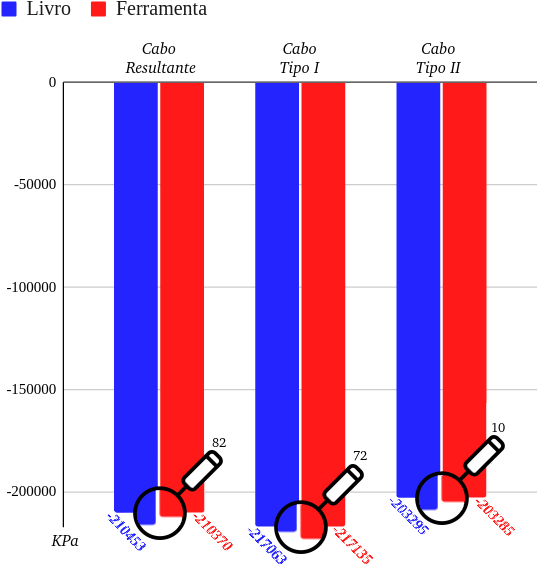
\includegraphics[width=0.8\textwidth]{imgs/efe_con.png}
    \caption{Diagrama de forças considerando os resultados do livro e da ferramenta.}
    \label{fig:efe_con}
    \medskip
    \small Fonte: Elaboração Própria (2024).
\end{figure}

Na Tabela \ref{fig:efe_con} as diferenças absolutas variam de 10 KPa a 83 KPa, com diferenças relativas máximas de 0,0394\%, o que evidencia mais uma vez, a concordância muito próxima que há entre os valores do livro e da ferramenta.

\newpage

\subsubsection{Exemplo de aplicação numérica para cálculo de relaxação pura e relativa}

\hspace{0.4cm}A aplicação numérica para a relaxação pura e relativa apresenta-se como a determinação destas a partir de um determinado processo de cálculo de perdas progressivas (Cholfe e Bonilha, \citeyear{CB}, p. 192). A relaxação pura resultante do livro foi de 70,51 MPa, e a da ferramenta foi de 70,42 MPa, resultando em uma diferença absoluta de 0,09 MPa e uma diferença relativa de 0,13\%. Já quanto à relaxação relativa, tem-se o valor do livro como de 46,63 MPa, enquanto o valor da ferramenta foi de 46,57 MPa, com em uma diferença absoluta de 0,06 MPa e uma diferença relativa também de 0,13\%, ou seja, resultados muito próximos, e consistentes com os exemplos anteriores.

\subsubsection{Exemplo de aplicação numérica para cálculo de perdas progressivas de protensão pelo método geral e processo simplificado}

\hspace{0.4cm}Chegando à aplicação numérica dos cálculos definitivos da perda de protensão progressiva, têm-se também uma viga protendida com aderência posterior e solicitada além da protensão por determinados momentos permanente e variável de acordo com o especificado na questão. Assim sendo, pede-se para determinar as perdas de protensão progressivas com efeitos da retração, fluência e relaxação a tempo infinito para um cabo resultante (Cholfe e Bonilha, \citeyear{CB}, p. 197). 

No cálculo para o presente trabalho, foram considerados o método geral e o processo simplificado, onde no primeiro o livro obteve o valor de -207979 KPa, semelhante ao da ferramenta, com nenhuma diferença absoluta e relativa. Continuando, para o processo simplificado, observa-se uma diferença absoluta entre o valor obtido pelo livro de -189108 KPa e o valor calculado pela ferramenta de -188164 KPa, o que representa uma diferença de aproximadamente 944 KPa. Em termos de diferença relativa, isso representa cerca de 0,5\%.

De modo geral, em todas as aplicações numéricas, as diferenças relativas ficaram abaixo de 1\%, exceto para retração e fluência, que apresentaram valores inferiores a 10\%. Isso indica que não houve nenhuma diferença absoluta significativa, o que permite atribuir essas variações a diferenças de aproximação. Esse argumento se fortalece principalmente porque os resultados com maiores diferenças são aqueles que dependem de pré-cálculos, como as perdas progressivas, que, para serem obtidas, exigem cálculos auxiliares. Esse acúmulo de aproximações gera, portanto, variações finais mais elevadas.

